\section{Parsing and Generating Code} % (fold)
\label{sec:parsing_and_generating}
This section gives a brief overview of what parsers are and how they work.

In a nutshell, a parser takes a file containing some text written in some syntax, and produces an abstract syntax tree. An abstract syntax tree is simply a more structured representation of the text, and is constructed using the rules of the syntax and the semantics of the language. 

We can use the abstract syntax tree to produce code in another language. For example, a compiler uses it to produce machine code. A \emph{transpiler} uses it to produce source code in another language.

\begin{figure}[ht]
  \centering
  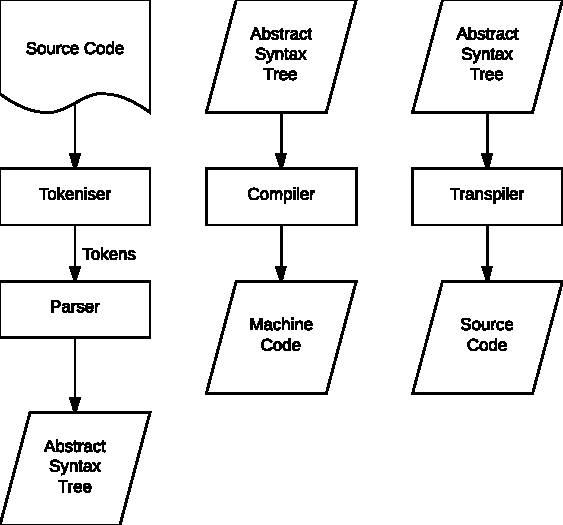
\includegraphics[width=0.65\textwidth]{parsers-compilers.pdf} 
  \caption{Flow charts showing the role of a parser, compiler and transpiler.}
  \label{fig:parsers-compilers}
\end{figure}

% section parsing_and_generating (end)